%OPERAZIONE DI GRUPPO
\begin{figure}[h]
	\centering
	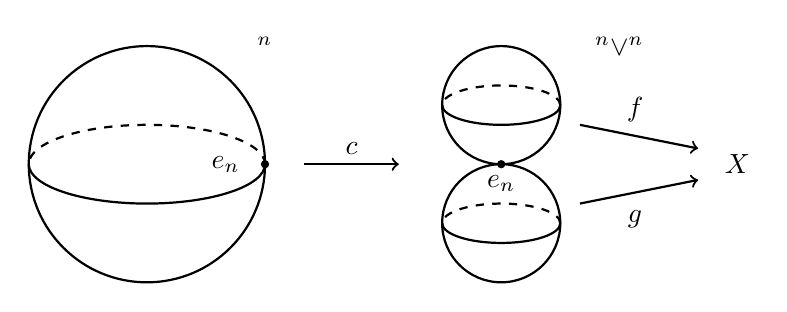
\begin{tikzpicture}
		%\draw[help lines](-2,-2) grid (10,2);
		
		%Sfera
		\draw[thick](-1.5,0)arc(180:360:1.5 and 0.5);
		\draw[thick,dashed](1.5,0)arc(0:180:1.5 and 0.5);
		\draw[thick] (0,0)circle(1.5);
		\fill (1.5,0) circle (1.5pt);
		\node at (1,0){\(e_n\)};
		\node at (1.5,1.5){\(\Sp^n\)};
		
		\draw [thick,->] (2,0)--(3.2,0);
		\node at (2.6,0.2){\(c\)};
		
		%Bouqet di sfere
		\draw[thick] (4.5,0.75)circle(0.75)
		(4.5,-0.75)circle(0.75);
		\draw[thick](3.75,0.75)arc(180:360:0.75 and 0.25)
		(3.75,-0.75)arc(180:360:0.75 and 0.25);
		\draw[thick,dashed](5.25,0.75)arc(0:180:0.75 and 0.25)
		(5.25,-0.75)arc(0:180:0.75 and 0.25);
		\fill (4.5,0) circle (1.5pt);	
		\node at (4.5,-0.25){\(e_n\)};
		\node at (6,1.5){\(\Sp^n \vee \Sp^n\)};
		
		\draw[thick,->](5.5,0.5)--(7,0.2);
		\draw[thick,->](5.5,-0.5)--(7,-0.2);
		
		\node at (6.2,0.7){\(f\)};
		\node at (6.2,-0.7){\(g\)};
		
		%X
		\node at(7.5,0){\(X\)};
	\end{tikzpicture}
	
	\caption{Operazione di gruppo su \(\pi_n(X,x_0)\).}
	\label{fig: operazione gruppo di omotopia}
\end{figure}